\documentclass[12pt]{article}
\newenvironment{problem}[2][Problem]{\begin{trivlist}
\item[\hskip \labelsep {\bfseries #1}\hskip \labelsep {\bfseries #2.}]}{\end{trivlist}}
\usepackage{amssymb}
\usepackage{amsmath}
\usepackage{fancyhdr}

\usepackage{graphicx}

\usepackage{etoolbox,refcount}
\usepackage{multicol}

\newcounter{countitems}
\newcounter{nextitemizecount}
\newcommand{\setupcountitems}{%
  \stepcounter{nextitemizecount}%
  \setcounter{countitems}{0}%
  \preto\item{\stepcounter{countitems}}%
}
\makeatletter
\newcommand{\computecountitems}{%
  \edef\@currentlabel{\number\c@countitems}%
  \label{countitems@\number\numexpr\value{nextitemizecount}-1\relax}%
}
\newcommand{\nextitemizecount}{%
  \getrefnumber{countitems@\number\c@nextitemizecount}%
}
\newcommand{\previtemizecount}{%
  \getrefnumber{countitems@\number\numexpr\value{nextitemizecount}-1\relax}%
}
\makeatother    
\newenvironment{AutoMultiColItemize}{%
\ifnumcomp{\nextitemizecount}{>}{3}{\begin{multicols}{2}}{}%
\setupcountitems\begin{itemize}}%
{\end{itemize}%
\unskip\computecountitems\ifnumcomp{\previtemizecount}{>}{3}{\end{multicols}}{}}


% \begin{itemize}
%     \item Here are two columns
%   \begin{AutoMultiColItemize}
%   \item Item 1
%   \item Item 2
%   \item Item 3
%   \item Item 4
%   \item Item 5
%   \item Item 6
%   \end{AutoMultiColItemize}
%   \item AutoMultiColItemize can be nested in an itemize
%   \item Or it does not have to be.
%   \item Normal itemize, like this one, are still single column.
% \end{itemize}
% Here is one column
% \begin{AutoMultiColItemize}
% \item Item 1
% \item Item 2
% \item Item 3
% \end{AutoMultiColItemize}


\begin{document}

\pagestyle{fancy}
\fancyhf{}
\lhead{GEOL 362A -- PS 1}
\rhead{Due: 24 Sept 2021}

% \title{Problem Set 1}
% % \author{GEOL 362A, Middlebury College}
% % \date{Due: 24 Sept 2021}
% \maketitle

\noindent The goal of this problem set is to get everyone on the same page with basic mathematical description of a glacier.  These problems will draw on van der Veen Chapter 1, some mathematical background from other courses, and concepts we discuss in lecture.

\begin{problem}{1}
[2 pts] For each of the following, write whether it is a scalar, vector, or tensor variable and how you know.

\renewcommand{\labelenumi}{(\alph{enumi})}
\begin{enumerate}
\setlength\itemsep{0.2em}
\begin{AutoMultiColItemize}
    \item Glacier velocity
    \item Cauchy stress
    \item Crevasse depth
    \item Hydrostatic pressure
    \item Surface mass balance
    \item Change in glacier front position
\end{AutoMultiColItemize}
\end{enumerate}
\end{problem}

%%%%%
\begin{problem}{2}
[2 pts] Notation: write out each of the following expressions in the notation given in van der Veen.
\renewcommand{\labelenumi}{(\alph{enumi})}
\begin{enumerate}
\setlength\itemsep{0.2em}
    \item The derivative of the $x$-component of velocity in the $x$ direction
    \item The components of the strain-rate tensor $\dot{\varepsilon}_{ij}$ (see Equation 1.34)
\end{enumerate}
\end{problem}

%%%%%
\begin{problem}{3}
[3 pts] Leigh and Denis are monitoring the motion of Helheim Glacier.  In March, they place two GPS stations on the ice surface, one at point A and one at point B.  In December of the same year, a transmission shows that the stations have moved to locations A’ and B’.

\begin{figure}
    \centering
    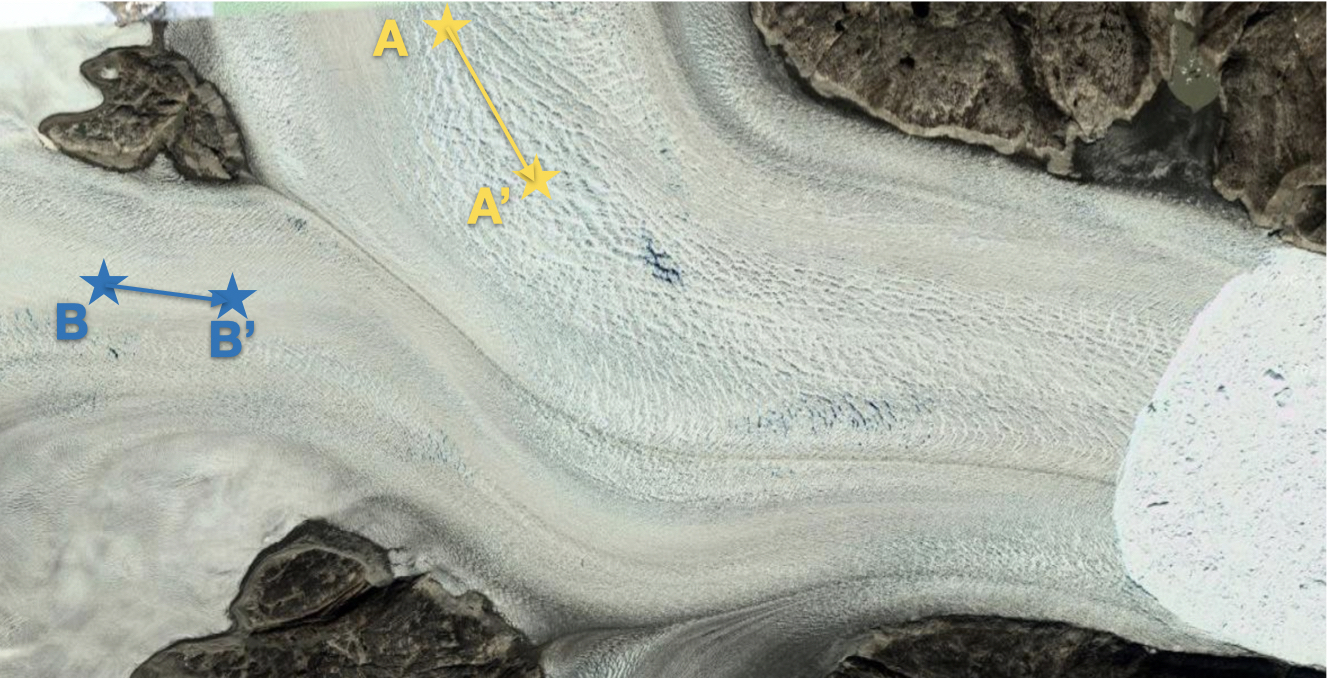
\includegraphics[width=1.0\linewidth]{figs/PS1-Helheim plot.jpeg}
    \caption{Stations A and B on Helheim Glacier.  Positions, in kilometers easting and northing, are A: (298, -2573); A': (300, -2578); B: (295, -2578); B': (297, -2579).}
    \label{fig:helheim}
\end{figure}


Find:
\renewcommand{\labelenumi}{(\alph{enumi})}
\begin{enumerate}
\setlength\itemsep{0.2em}
    \item The displacement vectors $\overrightarrow{AA’}$, $\overrightarrow{BB’}$.
    \item The velocity vectors of stations A and B
    \item The average speed recorded at the two stations over the period
\end{enumerate}


\end{problem}

\begin{problem}{4}
[3 pts] Consider the idealized glacier drawn below.  It has a constant mass balance gradient $\alpha$, such that the mass balance $a = \alpha (h-z_0)$ is positive above the equilibrium line elevation and negative below.

\begin{figure}
    \centering
    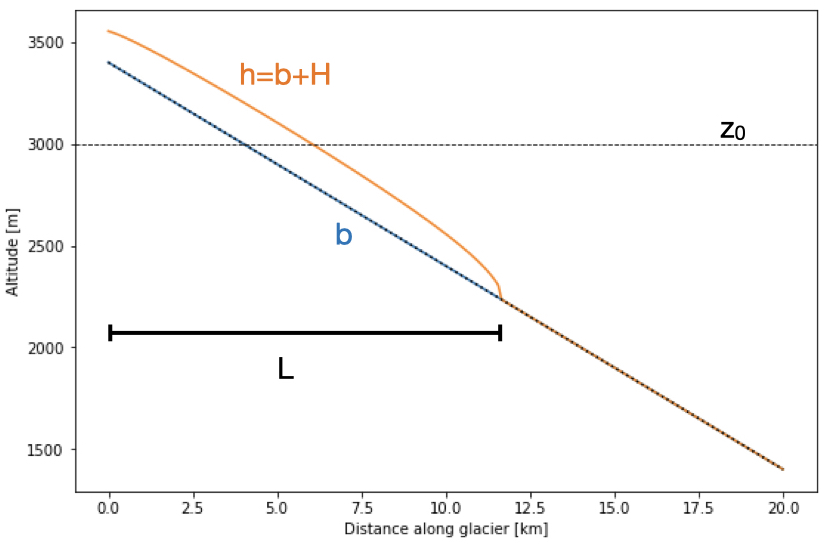
\includegraphics[width=0.8\linewidth]{figs/PS1-idealized_plot.jpeg}
    \caption{An idealized glacier of length $L$ with bed elevation $b$, surface elevation $h$, ice thickness $H$, and equilibrium line elevation $z_0$.  You may assume the width is constant and treat the problem along the cross-section shown.}
    \label{fig:idealized}
\end{figure}

\renewcommand{\labelenumi}{(\alph{enumi})}
\begin{enumerate}
\setlength\itemsep{0.2em}
    \item  Assuming the glacier is in equilibrium with its surroundings (no net flux in or out), write an equation for its conservation of mass.
    \item How does this change if we assume that the glacier is not in equilibrium?  For example, say that there is a net annual mass loss from the system?
\end{enumerate}

\end{problem}
\end{document}